\label{sec:complexity}

As discussed in Section \ref{sec:intro} the goal of the soft margins in the SVM is to maximize the margins while softly penalizes data points that lies in the wrong side of the margins borders.
The problem to be minimized is the following:
\begin{equation}
  0.5 ||w||^2 + C \sum_{i=1}^{N}\xi_i,
\end{equation}
where $w$ is the hyper-plane, $\xi_i$ is the penalty for each datapoint and $C$ is the regularization parameter.
Low values for $C$ means that the model "allows" more data points lying between the margins, making them "softer".
On the other hand, higher values for $C$ make the margins "harder".
Some examples of how the margins looks like for different values of $C$ can be seen in Figure \ref{fig:svm}.
It is possible to observe the margins getting harder and harder (with less data points as between the margins) when $C$ is increased by powers of 10.

\begin{figure}[!htb]
\begin{center}
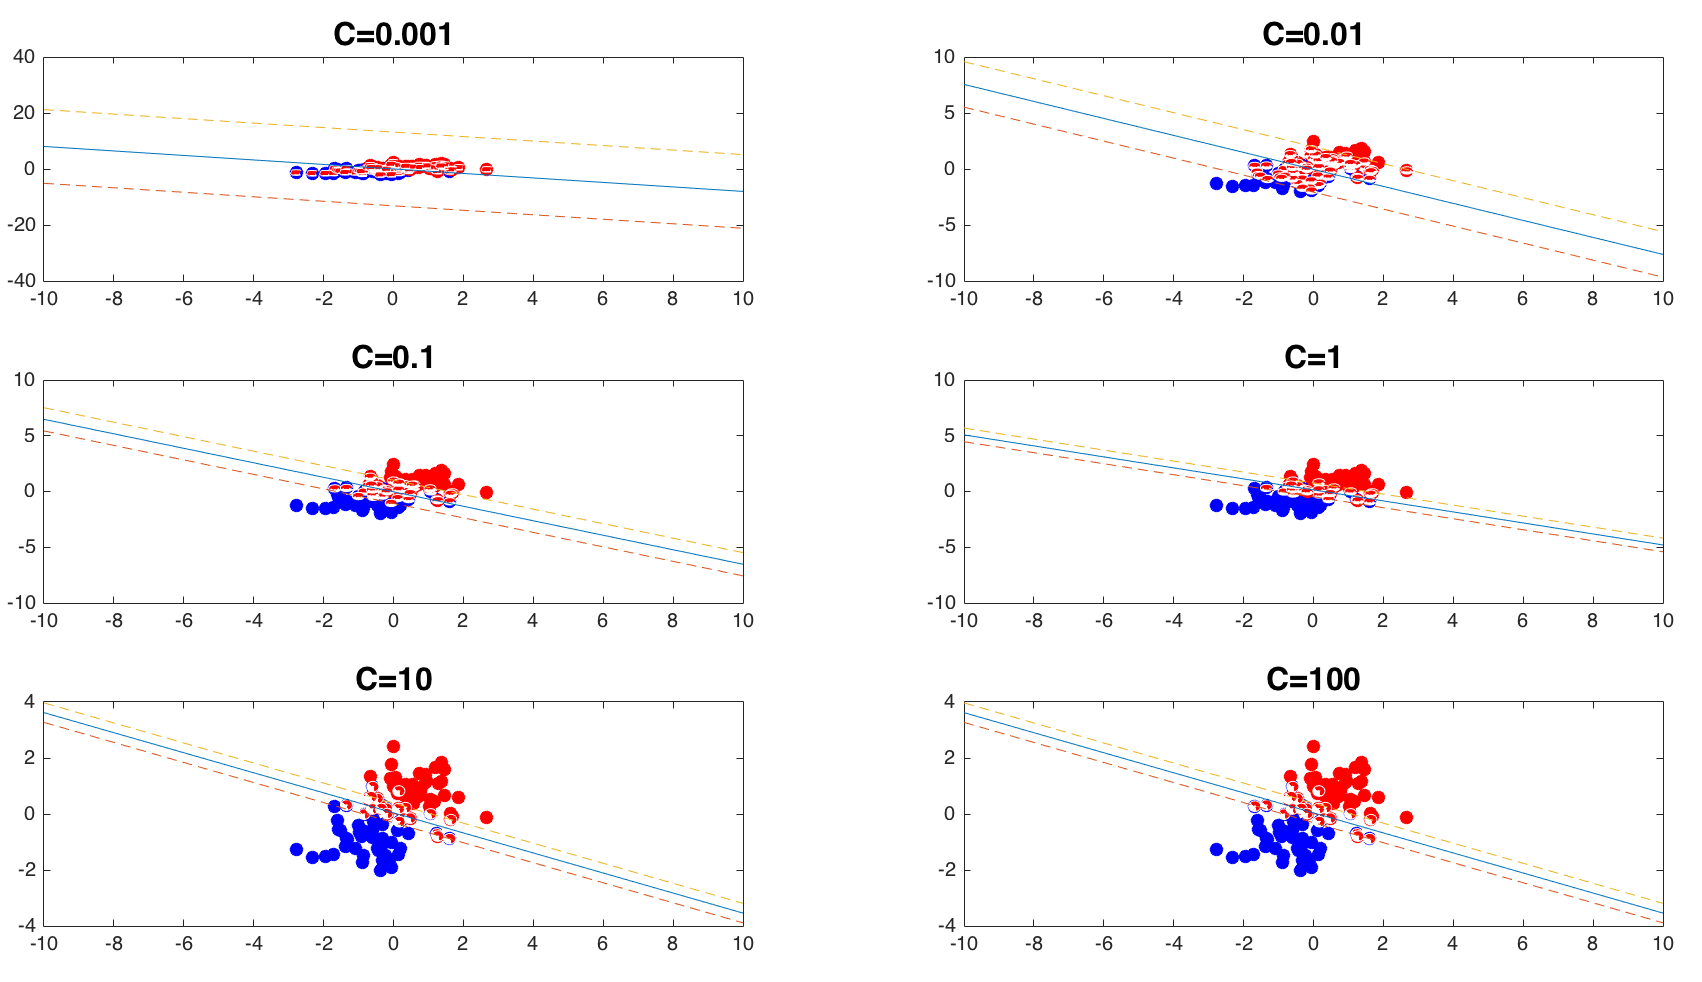
\includegraphics [width=10.5cm] {./graphics/SVM_PLOT.png}
\caption{Binary SVM under diferent values of $C$. The dashed circles in each subfigure are the support vectors.} \label{fig:svm}
\end{center}
\end{figure}

Since the strong duality holds for this QP problem, we can do some sensitive interpretations with the Lagrange variables.
The number of Lagrange variables greater than $0$ will gives us the number of support vectors.
The ratio $r$ between the number of support vectors and the number of data to train the SVM can gives us an intuition about the complexity of the model.
With $r$ equals to 1, means that the model needs the whole training data to define a decision boundary.
This makes our model more complex in the sense that the it needs as much active constraints as data.

The task of selection of $C$ is to select the most simple model that gives the highest accuracy.
Figure \ref{fig:toy} shows a plots of the training and test set accuracies (solid lines) and the value of $r$ (dashed line) for each value of $C$.

\begin{figure}[!htb]
\begin{center}
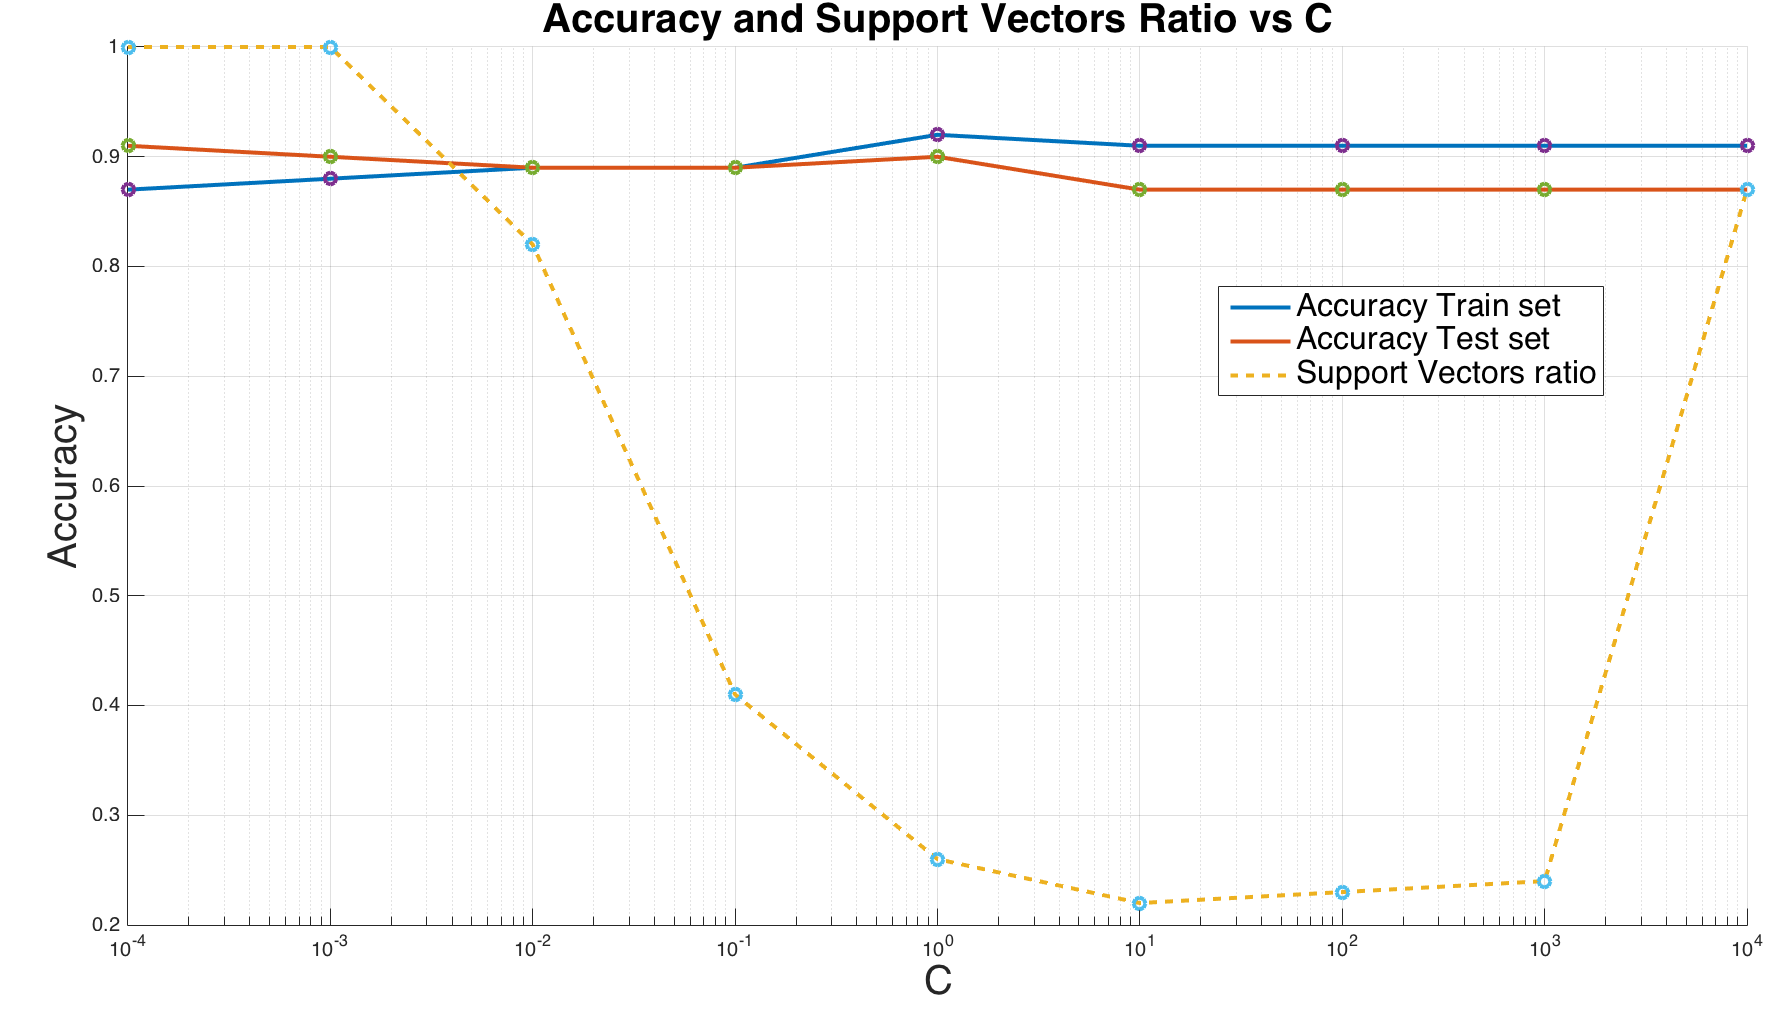
\includegraphics [width=10.5cm] {./graphics/toy_plot.png}
\caption{Accuracy and Support Vector Ratio $r$ vs $C$} \label{fig:toy}
\end{center}
\end{figure}

It is possible to observe that the accuracies are relatively stable along the range of $C$, but the models start to decrease complexity from $C=10^{-2}$.
A good trade-off between model complexity and accuracy can be reached with $C$ between $10^1$ and $10^3$ which corresponds $\approx 20\%$ of the training set as support vectors. 
The plots from Figures \ref{fig:svm} and \ref{fig:toy} can be reproduced executing the script called toy\_analysis.m .

The same sensitivity analysis can be done with real data.
Figure \ref{fig:datasets} shows the same Accuracy and $r$ plot for different values of $C$ for three different dataset.


Containing 150 data points slit in 3 classes the Iris Dataset \footnote{https://archive.ics.uci.edu/ml/datasets/iris} is a well known database used in the pattern recognition literature.
In Figure \ref{fig:datasets} (a) it is possible to observe that the good trade-off is obtained with $C=10^2$ with an accuracy above 90\% in the training set and in the test set.
The plot can be reproduced executing the script iris\_analysis.m.m .

Figure \ref{fig:datasets} (b) presents the same analysis with the Wine Dataset (178 data points split in 3 classes)\footnote{https://archive.ics.uci.edu/ml/datasets/wine}.
The good trade-off can be observed with $C$ greater than $1$ with an accuracy above 90\% for both training and test sets.
The plot can be reproduced executing the script wine\_analysis.m .

Finally Figure \ref{fig:datasets} (c) presents the analysis with the Column Vertebral Dataset \footnote{https://archive.ics.uci.edu/ml/datasets/Vertebral+Column} (310 data points split in three classes).
The trade-off can be observed with $C$ equals to $10$ with an accuracy above 80\% for both training and test sets.
The plot can be reproduced executing the script vertebral\_column\_analysis.m .

\begin{figure}[!htb]
\begin{center}
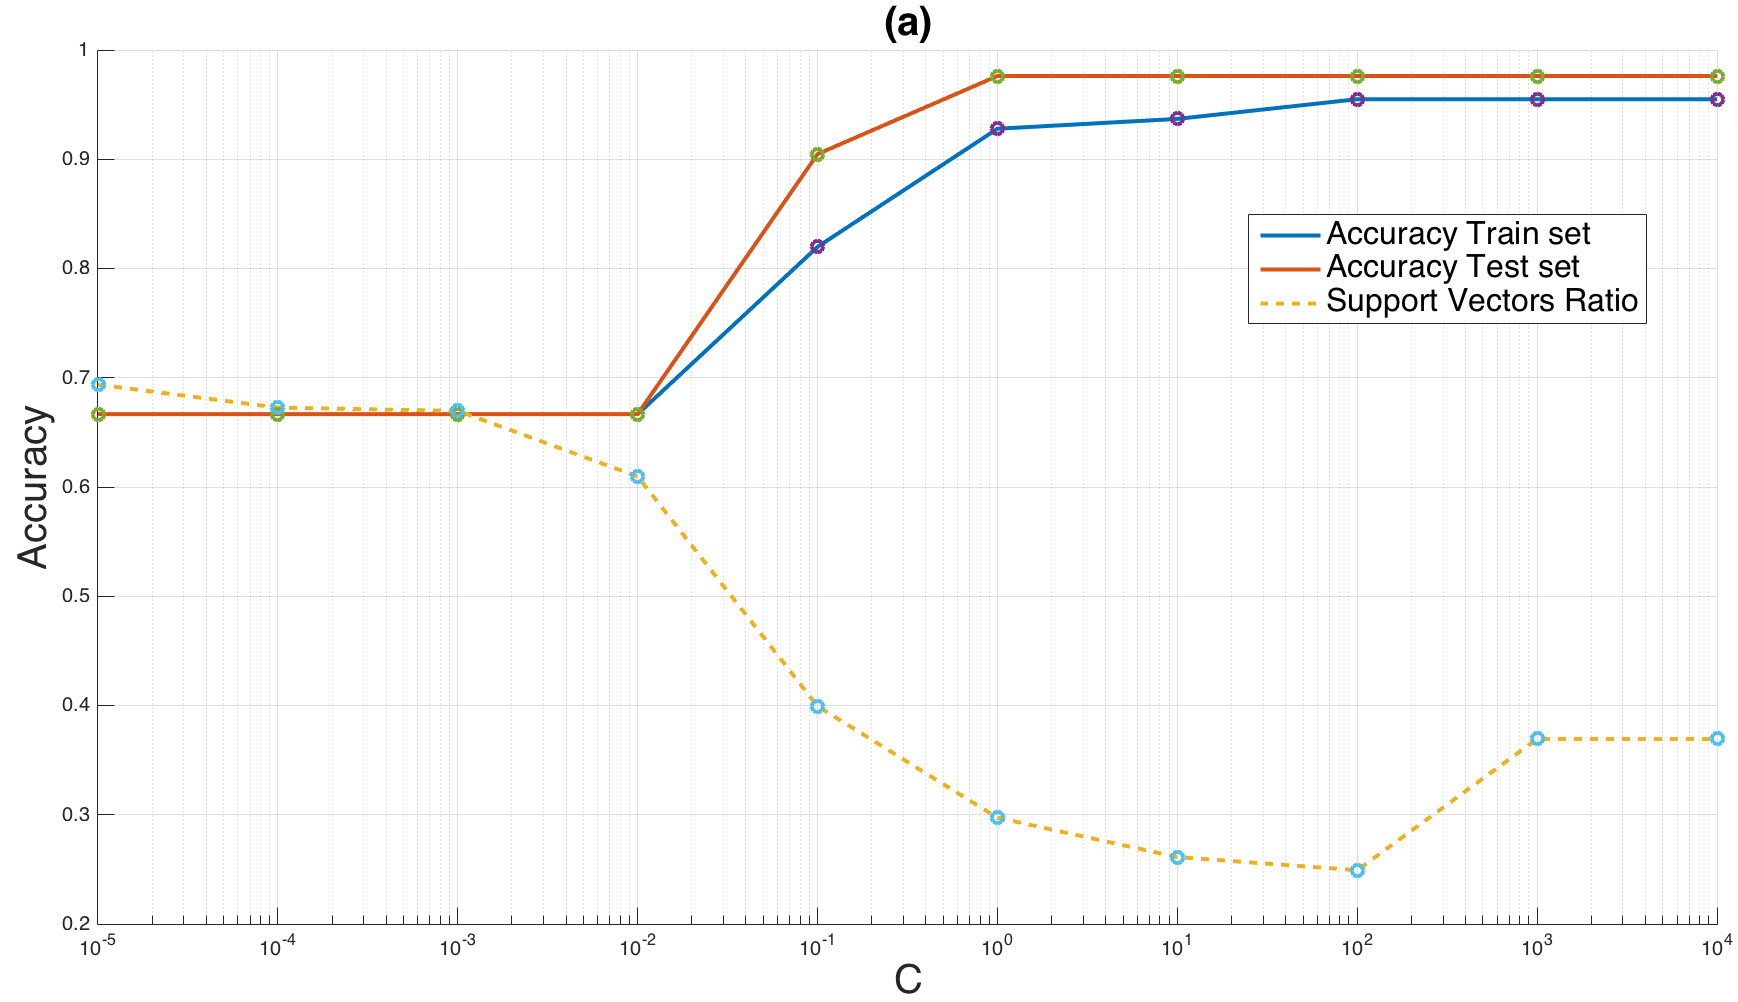
\includegraphics [width=8.5cm] {./graphics/iris.png}
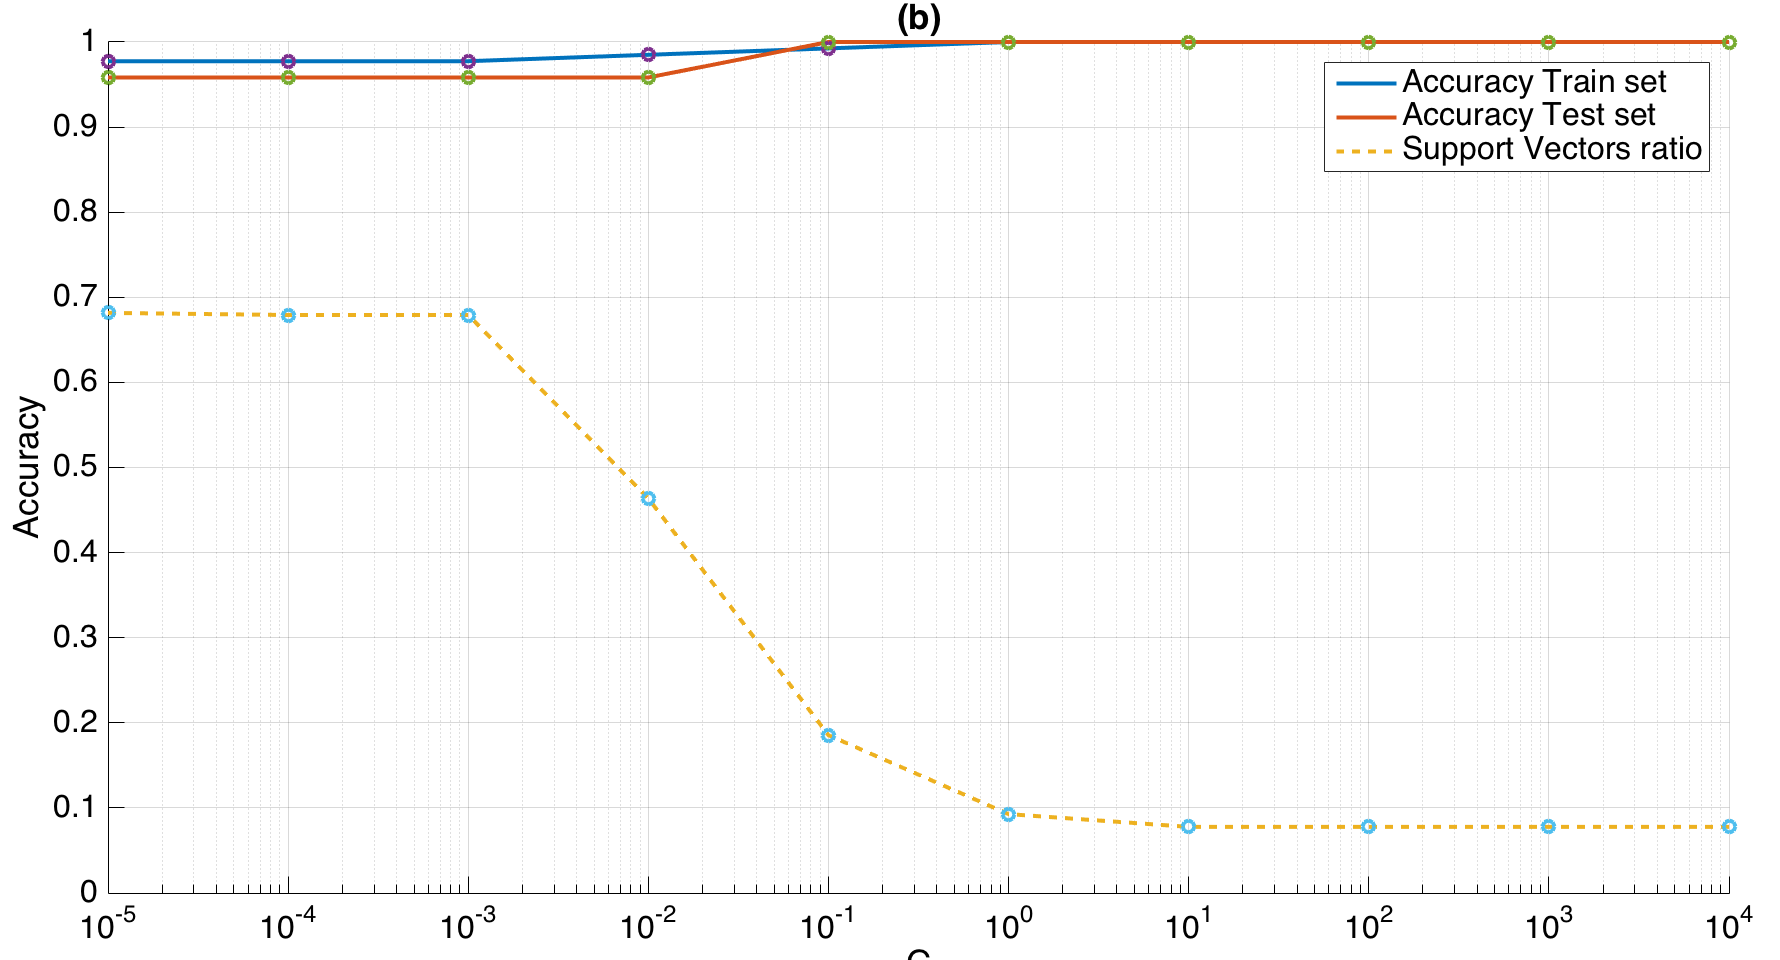
\includegraphics [width=8.5cm] {./graphics/wine.png}

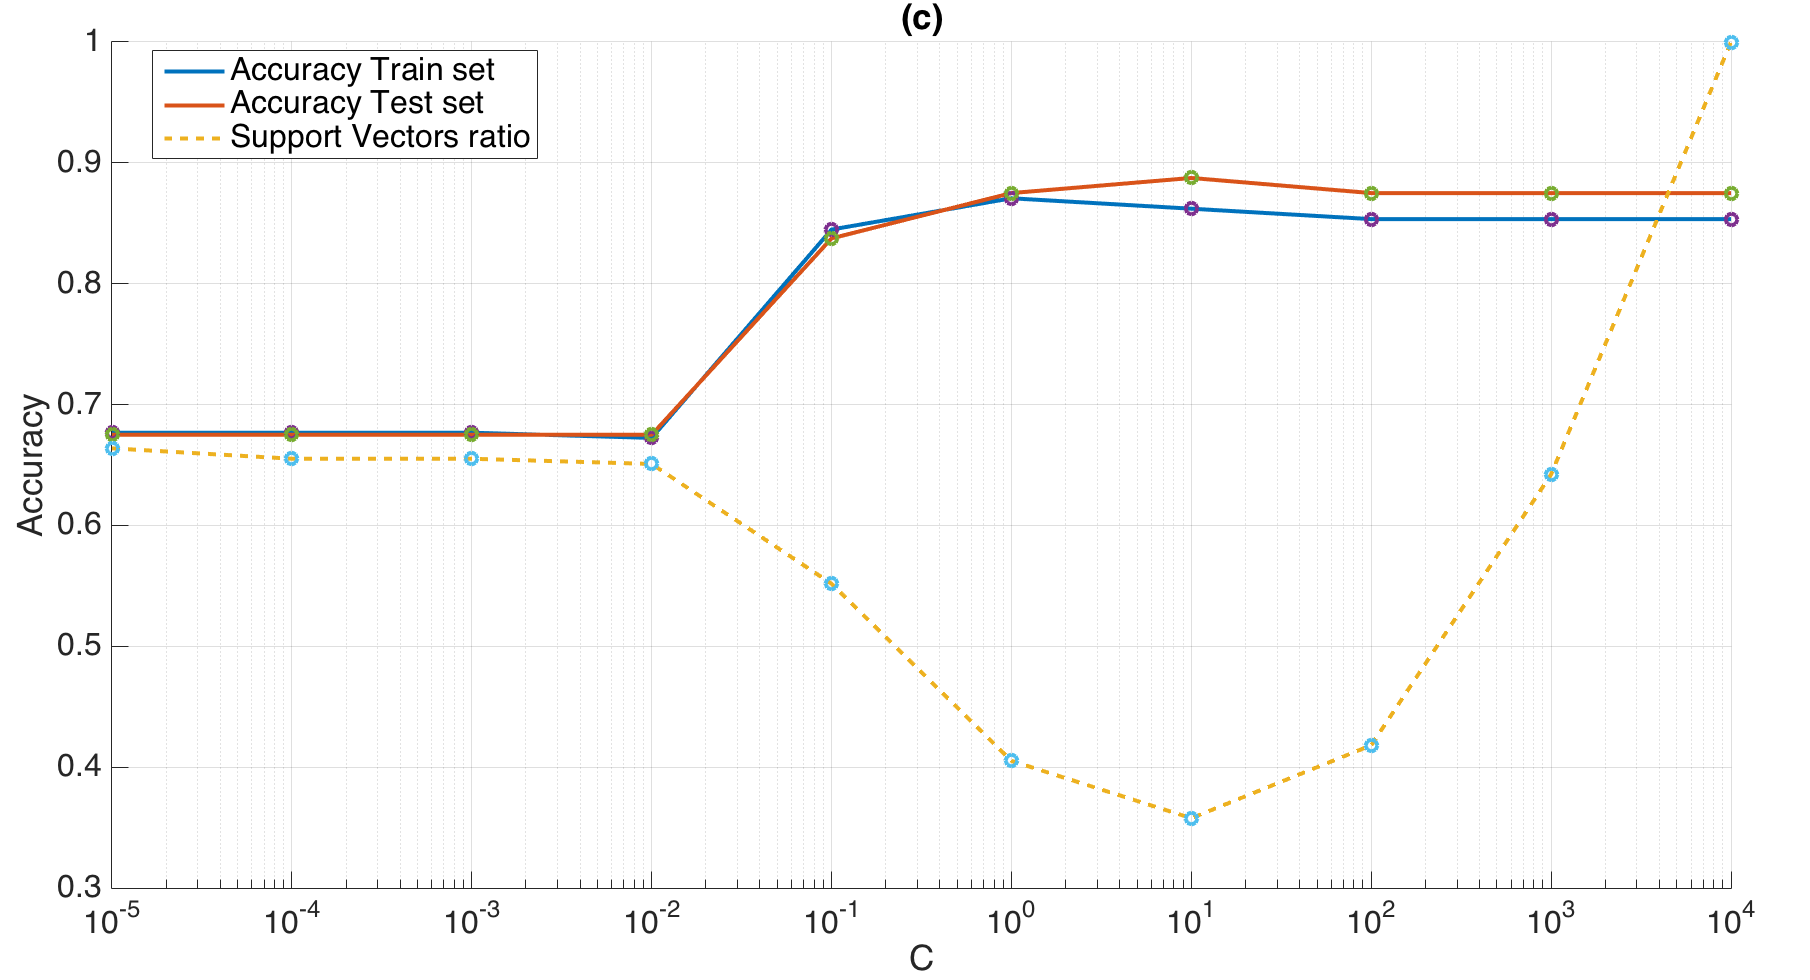
\includegraphics [width=8.5cm] {./graphics/vertebral_column.png}
\caption{Accuracy and Support Vector Ratio $r$ vs $C$ for the Iris (a), Wine (b) and Column Vertebral Dataset (c)} \label{fig:datasets}
\end{center}
\end{figure}



